\section{Liên trường Đà Nẵng, Lần 1, NH: 25-26}

\caulc
\Opensolutionfile{ans}[ans/ans-19-26-2-DaNang-LienTruong-L1-LC]
%%%=============EX_1=============%%%
\begin{ex}%[0D0H2-7]%[TEX ĐỀ THI THỬ THPT 2026]%[NGUYỄN VĂN HIỆP]
	Một hộp chứa $10$ tấm thẻ cùng loại được đánh số từ $1$ đến $10$. Bạn Bình lấy ra lần lượt $2$ tấm thẻ từ hộp. Thẻ lấy ra lần thứ nhất không được trả lại hộp. Xác suất của biến cố \lq\lq Tổng các số trên $2$ tấm thẻ bằng $12$\rq\rq\, bằng
	\choice
	{$\dfrac{1}{12}$}
	{$\dfrac{1}{10}$}
	{$\dfrac{2}{15}$}
	{\True $\dfrac{4}{45}$}
	\loigiai{
		Số phần tử của không gian mẫu $n(\Omega)=\mathrm{A}_{10}^2=90$.\\
		Gọi $A$ là biến cố \lq\lq Tổng các số trên $2$ tấm thẻ bằng $12$\rq\rq.\\
		Các cặp thẻ lấy ra có tổng bằng $12$ là $(2; 10)$, $(10; 2)$, $(3; 9)$, $(9; 3)$, $(4; 8)$, $(8; 4)$, $(5; 7)$, $(7; 5)$.
		Suy ra $n(A)=8$.\\
		Xác suất của biến cố $A$ là $\mathrm{P}(A)=\dfrac{n(A)}{n(\Omega)}=\dfrac{8}{90}=\dfrac{4}{45}$.
	}
\end{ex}
%%%=============================%%%

%%%=============EX_2=============%%%
\begin{ex}%[1D6H4-4]%[TEX ĐỀ THI THỬ THPT 2026]%[NGUYỄN VĂN HIỆP]
	Số nghiệm của phương trình $\log_2(x-4)=\log_2(x^2-5x+4)$ là
	\choice
	{$1$}
	{$2$}
	{\True $0$}
	{$3$}
	\loigiai{
		Điều kiện xác định $x-4>0\Leftrightarrow x>4$.\\
		Phương trình đã cho tương đương với
		\[ x-4=x^2-5x+4\Leftrightarrow x^2-6x+8=0\Leftrightarrow\hoac{&x=2\\&x=4.}\]
		Đối chiếu điều kiện, ta thấy cả hai nghiệm đều không thỏa mãn.\\
		Vậy phương trình đã cho vô nghiệm.
	}
\end{ex}
%%%=============================%%%

%%%=============EX_3=============%%%
\begin{ex}%[2D1N4-1]%[TEX ĐỀ THI THỬ THPT 2026]%[NGUYỄN VĂN HIỆP]
	\immini{
	Cho hàm số $y=f(x)$ có bảng biến thiên như sau
	Đường tiệm cận đứng, tiệm cận ngang của đồ thị hàm số đã cho lần lượt là
	\choice
	{$x=1$; $y=2$}
	{\True $x=2$; $y=1$}
	{$x=2$; $y=2$}
	{$x=1$; $y=1$}
	}{
		
\begin{tikzpicture}[font=\footnotesize, line join=round, line cap=round, >=stealth]
			\tkzTabInit[nocadre=false, lgt=1.2, espcl=1.6, deltacl=0.5]
			{$x$ / 0.6, $f'(x)$ / 0.6, $f(x)$ / 2}
			{$-\infty$, $2$, $+\infty$}
			\tkzTabLine{, -, d, -, }
			\tkzTabVar{+/ $1$, -D+/ $-\infty$ / $+\infty$, -/ $1$}
		\end{tikzpicture}
	}
	\loigiai{
		Dựa vào bảng biến thiên, ta có
		\begin{itemize}
			\item $\lim\limits_{x\to 2^-}f(x)=-\infty$ và $\lim\limits_{x\to 2^+}f(x)=+\infty$ nên đường thẳng $x=2$ là tiệm cận đứng.
			\item $\lim\limits_{x\to-\infty}f(x)=1$ và $\lim\limits_{x\to+\infty}f(x)=1$ nên đường thẳng $y=1$ là tiệm cận ngang.
		\end{itemize}
	}
\end{ex}
%%%=============================%%%

%%%=============EX_4=============%%%
\begin{ex}%[2H2N2-2]%[TEX ĐỀ THI THỬ THPT 2026]%[NGUYỄN VĂN HIỆP]
	Trong không gian $Oxyz$, cho điểm $A(3; 2;-5)$ và $B$ là điểm đối xứng của $A$ qua mặt phẳng $(Oyz)$. Tọa độ điểm $B$ là
	\choice
	{\True $(-3; 2;-5)$}
	{$(0; 2;-5)$}
	{$(3;-2; 5)$}
	{$(3; 0; 0)$}
	\loigiai{
		Điểm đối xứng của điểm $M(x; y; z)$ qua mặt phẳng $(Oyz)$ có tọa độ là $(-x; y; z)$.\\
		Do đó, điểm đối xứng của $A(3; 2;-5)$ qua mặt phẳng $(Oyz)$ là $B(-3; 2;-5)$.
	}
\end{ex}
%%%=============================%%%

%%%=============EX_5=============%%%
\begin{ex}%[2D1H1-1]%[TEX ĐỀ THI THỬ THPT 2026]%[NGUYỄN VĂN HIỆP]
	Cho hàm số $y=f(x)$ có đạo hàm $f'(x)=x(4-x)$ với mọi $x\in\mathbb{R}$. Khẳng định nào sau đây đúng?
	\choice
	{$f(3)>f(4)$}
	{$f(5)<f(6)$}
	{$f(0)>f(2)$}
	{\True $f(-1)>f(0)$}
	\loigiai{
		Ta có $f'(x)=0\Leftrightarrow x(4-x)=0\Leftrightarrow\hoac{&x=0\\&x=4.}$\\
		Lập bảng xét dấu đạo hàm
		\begin{center}
			
\begin{tikzpicture}[font=\footnotesize, line join=round, line cap=round, >=stealth]
				\tkzTabInit[nocadre=false, lgt=1.2, espcl=3, deltacl=0.5]
				{$x$ / 0.6, $f'(x)$ / 0.6}
				{$-\infty$, $0$, $4$, $+\infty$}
				\tkzTabLine{, -, 0, +, 0, -, }
			\end{tikzpicture}
		\end{center}
		Ta thấy hàm số nghịch biến trên các khoảng $(-\infty; 0)$ và $(4;+\infty)$, đồng biến trên khoảng $(0; 4)$.\\
		Vì $-1<0$ và thuộc khoảng nghịch biến $(-\infty; 0)$ nên $f(-1)>f(0)$.
	}
\end{ex}
%%%=============================%%%

%%%=============EX_6=============%%%
\begin{ex}%[1D5H1-3]%[TEX ĐỀ THI THỬ THPT 2026]%[NGUYỄN VĂN HIỆP]
	Để chuẩn bị cho tiết học \lq\lq Mạng xã hội: lợi và hại\rq\rq\, (hoạt động thực hành trải nghiệm môn Toán, lớp $10$), cô A đã khảo sát thời gian sử dụng mạng xã hội trong một ngày của học sinh trong lớp $10$B và thu được mẫu số liệu ghép nhóm như sau
	\begin{center}
		\begin{tabular}{|c|c|c|c|c|c|c|}
			\hline
			Thời gian sử dụng \\  mạng xã hội (phút) & $[10; 20)$ & $[20; 30)$ & $[30; 40)$ & $[40; 50)$ & $[50; 60)$ & $[60; 70)$ \\
			\hline
			\textbf{Số học sinh} & $5$ & $7$ & $15$ & $6$ & $5$ & $4$ \\
			\hline
		\end{tabular}
	\end{center}
	Thời gian trung bình sử dụng mạng xã hội trong một ngày của học sinh lớp $10$B xấp xỉ bằng
	\choice
	{$38$}
	{$32{,}6$}
	{$36{,}7$}
	{\True $37{,}6$}
	\loigiai{
		Chọn giá trị đại diện cho mỗi nhóm là trung bình cộng của hai đầu mút, ta có các giá trị đại diện lần lượt là $15$, $25$, $35$, $45$, $55$, $65$.\\
		Cỡ mẫu $n=5+7+15+6+5+4=42$.\\
		Thời gian trung bình là
		\[\overline{x}=\dfrac{15\cdot 5+25\cdot 7+35\cdot 15+45\cdot 6+55\cdot 5+65\cdot 4}{42}=\dfrac{1\,580}{42}\approx 37{,}6. \]
	}
\end{ex}
%%%=============================%%%

%%%=============EX_7=============%%%
\begin{ex}%[2D1H5-1]%[TEX ĐỀ THI THỬ THPT 2026]%[NGUYỄN VĂN HIỆP]
	\immini[thm]
	{
		Đường cong cho trong hình vẽ bên là đồ thị của hàm số nào trong các hàm số dưới đây?
		\choice
		{\True $y=x^3-3x+1$}
		{$y=2x^3-6x+1$}
		{$y=-x^3+3x+1$}
		{$y=-x^3+2x-1$}
	}
	{
		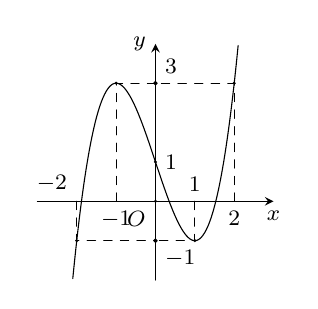
\begin{tikzpicture}[scale=0.5, font=\footnotesize, line join=round, line cap=round, >=stealth]
			\draw[->] (-3,0) -- (3,0) node[below] {$x$};
			\draw[->] (0,-2) -- (0,4) node[left] {$y$};
			\fill (0,0) node[below left] {$O$} circle (1.2pt);
			\draw[smooth, samples=100, domain=-2.1:2.1] plot(\x, {(\x)^3 - 3*(\x) + 1});
			\fill (-1,3) circle (1.2pt);
			\fill (1,-1) circle (1.2pt);
			\fill (0,1) circle (1.2pt);
			\fill (-2,-1) circle (1.2pt);
			\fill (2,3) circle (1.2pt);
			\draw[dashed] (-1,0) node[below]{$-1$} -- (-1,3) -- (0,3) node[above right]{$3$};
			\draw[dashed] (1,0) node[above]{$1$} -- (1,-1) -- (0,-1) node[below right]{$-1$};
			\draw[fill=black] (0,-1) circle (1.2pt);
			\draw[fill=black] (0,3) circle (1.2pt);
			\draw[dashed] (-2,0) node[above left]{$-2$} -- (-2,-1) -- (0,-1);
			\draw[dashed] (2,0) node[below]{$2$} -- (2,3) -- (0,3);
			\draw (0,1) node[right]{$1$};
		\end{tikzpicture}
	}
	\loigiai{
		Dựa vào hình dáng đồ thị, ta thấy nhánh ngoài cùng bên phải hướng lên nên hệ số $a>0$.\\
		Loại C. $y=-x^3+3x+1$ và D. $y=-x^3+2x-1$.\\
		Đồ thị hàm số đi qua điểm $(1;-1)$.\\
		Thay $x=1$ vào $y=x^3-3x+1$ ta được $y=-1$ (thỏa mãn).\\
		Thay $x=1$ vào $y=2x^3-6x+1$ ta được $y=-3\neq-1$ (loại).\\
		Vậy hàm số cần tìm là $y=x^3-3x+1$.
	}
\end{ex}
%%%=============================%%%

%%%=============EX_8=============%%%
\begin{ex}%[2H2H1-2]%[TEX ĐỀ THI THỬ THPT 2026]%[NGUYỄN VĂN HIỆP]
	\immini[thm]
	{
		Cho hình hộp $ABCD.A'B'C'D'$. Mệnh đề nào dưới đây là \textbf{sai}?
		\choice
		{\True $\overrightarrow{AB'}+\overrightarrow{BC}=\overrightarrow{AC}$}
		{$\overrightarrow{AC}+\overrightarrow{DD'}=\overrightarrow{AC'}$}
		{$\overrightarrow{A'B'}+\overrightarrow{AD}=\overrightarrow{AC}$}
		{$\overrightarrow{AD}+\overrightarrow{CC'}=\overrightarrow{AD'}$}
	}
	{
		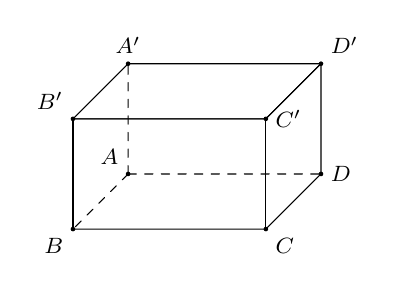
\begin{tikzpicture}[scale=0.7, font=\footnotesize, line join=round, line cap=round, >=stealth]
			\coordinate (A) at (1,1);
			\coordinate (B) at (0,0);
			\coordinate (C) at (3.5,0);
			\coordinate (D) at (4.5,1);
			\coordinate (A') at (1,3);
			\coordinate (B') at (0,2);
			\coordinate (C') at (3.5,2);
			\coordinate (D') at (4.5,3);
			\draw (B) node[below left]{$B$} -- (C) node[below right]{$C$} -- (D) node[right]{$D$} -- (D') node[above right]{$D'$} -- (C') node[right]{$C'$} -- (B') node[above left]{$B'$} -- cycle;
			\draw (B') -- (C') -- (D') -- (A') node[above]{$A'$} -- cycle;
			\draw (B) -- (B') (C) -- (C');
			\draw[dashed] (A) node[above left]{$A$} -- (B) (A) -- (D) (A) -- (A');
			\fill (A) circle (1.2pt) (B) circle (1.2pt) (C) circle (1.2pt) (D) circle (1.2pt);
			\fill (A') circle (1.2pt) (B') circle (1.2pt) (C') circle (1.2pt) (D') circle (1.2pt);
		\end{tikzpicture}
	}
	\loigiai{
		Xét mệnh đề A. $\overrightarrow{AB'}+\overrightarrow{BC}=\overrightarrow{AC}$.\\
		Ta có $VP=\overrightarrow{AB'}+\overrightarrow{BC}=\overrightarrow{AB'}+\overrightarrow{B'C'}=\overrightarrow{AC'}$. Do đó mệnh đề A sai.
	}
\end{ex}
%%%=============================%%%

%%%=============EX_9=============%%%
\begin{ex}%[2D1H3-1]%[TEX ĐỀ THI THỬ THPT 2026]%[NGUYỄN VĂN HIỆP]
	Giá trị lớn nhất của hàm số $f(x)=2\,026+2x-2\mathrm{e}^x$ trên đoạn $[0; 2]$ bằng
	\choice
	{$2\,026$}
	{\True $2\,024$}
	{$2\,028-2\mathrm{e}$}
	{$2\,030-2\mathrm{e}^2$}
	\loigiai{
		Hàm số đã cho liên tục trên đoạn $[0; 2]$.\\
		Đạo hàm $f'(x)=2-2\mathrm{e}^x$.\\
		Cho $f'(x)=0\Leftrightarrow\mathrm{e}^x=1\Leftrightarrow x=0\in[0; 2]$.\\
		Với mọi $x\in(0; 2]$, ta có $\mathrm{e}^x>1\Rightarrow f'(x)<0$.\\
		Do đó hàm số nghịch biến trên đoạn $[0; 2]$.\\
		Vậy $\max\limits_{x\in[0; 2]}f(x)=f(0)=2\,026+0-2\mathrm{e}^0=2\,024$.
	}
\end{ex}
%%%=============================%%%

%%%=============EX_10=============%%%
\begin{ex}%[2H2N2-1]%[TEX ĐỀ THI THỬ THPT 2026]%[NGUYỄN VĂN HIỆP]
	Trong không gian $Oxyz$, cho vectơ $\overrightarrow{a}=(3;-1; 2)$. Độ dài của vectơ $\overrightarrow{a}$ bằng
	\choice
	{$\sqrt{6}$}
	{\True $\sqrt{14}$}
	{$2$}
	{$4$}
	\loigiai{
		Độ dài của vectơ $\overrightarrow{a}$ là $\left|\overrightarrow{a}\right|=\sqrt{3^2+(-1)^2+2^2}=\sqrt{9+1+4}=\sqrt{14}$.
	}
\end{ex}
%%%=============================%%%

%%%=============EX_11=============%%%
\begin{ex}%[2D1N2-2]%[TEX ĐỀ THI THỬ THPT 2026]%[NGUYỄN VĂN HIỆP]
	\immini{
	Cho hàm số $f(x)$ có bảng biến thiên như hình vẽ dưới đây.Giá trị cực tiểu của hàm số đã cho là
	\choice
	{$3$}
	{$4$}
	{\True $-1$}
	{$-2$}
	}{
		
\begin{tikzpicture}[line join=round, line cap=round, >=stealth]
			\tkzTabInit[nocadre=false, lgt=1.2, espcl=1.6]
			{$x$ / 0.6, $f'(x)$ / 0.6, $f(x)$ / 2}
			{$-\infty$, $-2$, $3$, $+\infty$}
			\tkzTabLine{, +, 0, -, 0, +, }
			\tkzTabVar{-/ $-\infty$, +/ $4$, -/ $-1$, +/ $+\infty$}
		\end{tikzpicture}
	}
	\loigiai{
		Dựa vào bảng biến thiên, ta thấy hàm số đạt cực tiểu tại $x_{CT}=3$ và giá trị cực tiểu của hàm số là $y_{CT}=-1$.
	}
\end{ex}
%%%=============================%%%

%%%=============EX_12=============%%%
\begin{ex}%[2H2H2-3]%[TEX ĐỀ THI THỬ THPT 2026]%[NGUYỄN VĂN HIỆP]
	Trong không gian $Oxyz$, cho tam giác $MNP$ có $M(2; 3; 4)$, $N(-1; 2; 3)$ và $P(3; 2;-3)$. Vectơ $\overrightarrow{u}=2\overrightarrow{MN}-\overrightarrow{NP}$ có tọa độ là
	\choice
	{\True $(-10;-2; 4)$}
	{$(-2;-2;-4)$}
	{$(10; 2;-4)$}
	{$(5; 1;-2)$}
	\loigiai{
		Ta có $\overrightarrow{MN}=(-3;-1;-1)\Rightarrow 2\overrightarrow{MN}=(-6;-2;-2)$.\\
		Lại có $\overrightarrow{NP}=(4; 0;-6)$.\\
		Suy ra $\overrightarrow{u}=2\overrightarrow{MN}-\overrightarrow{NP}=(-6-4;-2-0;-2-(-6))=(-10;-2; 4)$.
	}
\end{ex}

\Closesolutionfile{ans}


\cauds
\Opensolutionfile{ans}[ans/ans-19-26-2-DaNang-LienTruong-L1-DS]
\begin{ex}%[2D1V3-6]%[TEX ĐỀ THI THỬ THPT 2026]%[NGUYỄN VĂN HIỆP]
	\immini[thm]{Cho một tấm nhôm hình vuông cạnh $12$ cm. Người ta cắt ở bốn góc của tấm nhôm đó bốn hình vuông bằng nhau, mỗi hình vuông có cạnh $x$ cm, rồi gấp tấm nhôm lại để được một cái hộp không nắp.
		\choiceTF
		{\True Độ dài cạnh đáy của cái hộp là $(12-2x)$ cm}
		{Thể tích cái hộp được tính theo công thức $V(x)=4x^3+144x$}
		{\True Đạo hàm của hàm thể tích là $V'(x)=12x^2-96x+144$}
		{\True Cái hộp có thể tích lớn nhất khi $x=2$}
	}{
		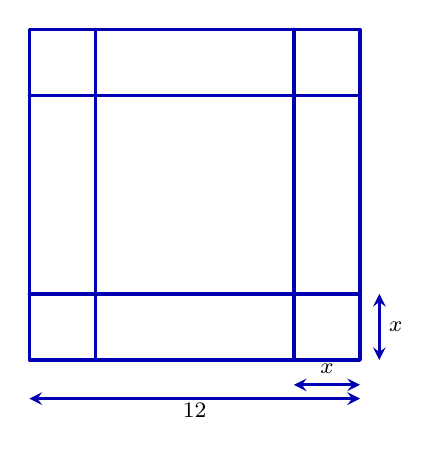
\begin{tikzpicture}[scale=0.7, line join=round, line cap=round,>=stealth,font=\footnotesize]
			\def\L{6}
			\def\t{1.2}
			
			% Hình vuông lớn
			\draw[blue!70!black, line width=1.2pt] (0,0) rectangle (\L,\L);
			
			% Hình vuông đáy
			\draw[blue!70!black, line width=1.2pt] (\t,\t) rectangle ({\L-\t},{\L-\t});
			
			% Các đoạn chia ở 4 góc
			\draw[blue!70!black, line width=1.2pt]
			(\t,0)--(\t,\t)
			({\L-\t},0)--({\L-\t},\t)
			(\t,\L)--(\t,{\L-\t})
			({\L-\t},\L)--({\L-\t},{\L-\t})
			(0,\t)--(\t,\t)
			(0,{\L-\t})--(\t,{\L-\t})
			(\L,\t)--({\L-\t},\t)
			(\L,{\L-\t})--({\L-\t},{\L-\t});
			
			% Kích thước 12
			\draw[blue!70!black, line width=1pt,<->] (0,-0.7)--(\L,-0.7);
			\node[below] at ({\L/2},-0.6) {$12$};
			
			% Kích thước x
			\draw[blue!70!black, line width=1pt,<->] (\L+0.35,0)--(\L+0.35,\t);
			\node[right] at (\L+0.35,{\t/2}) {$x$};
			
			\draw[blue!70!black, line width=1pt,<->] ({\L-\t},-0.45)--(\L,-0.45);
			\node[below] at ({\L-\t/2},0.1) {$x$};
		\end{tikzpicture}
	}
	\loigiai{
		\begin{itemchoice}
			\itemch Mỗi cạnh của tấm nhôm bị cắt đi hai đoạn dài $x$, nên cạnh đáy của hộp là $12-2x$, với $0<x<6$.
			\itemch Sau khi cắt và gấp, chiều cao của hộp là $x$ và đáy là hình vuông cạnh $12-2x$.\\
			Suy ra thể tích của hộp là
			$V(x)=x(12-2x)^2=4x^3-48x^2+144x$.
			\itemch Từ $V(x)=4x^3-48x^2+144x$,
			suy ra $V'(x)=12x^2-96x+144$.
			\itemch Ta có
			\[
			V'(x)=0 \Leftrightarrow 12x^2-96x+144=0
			\Leftrightarrow x^2-8x+12=0
			\Leftrightarrow \hoac{&x=2 \\&x=6.}
			\]
			Bảng biến thiên
			\begin{center}
				
\begin{tikzpicture}[scale=1,font=\footnotesize,line join=round
					,line cap=round,>=stealth]
					\tkzTabInit[nocadre=false, lgt=1.2,espcl=4, deltacl=0.5]
					{$x$/0.6,$V'(x)$/0.6,$V(x)$/2}
					{$0$, $2$, $6$}
					\tkzTabLine{,+,z,-}
					\tkzTabVar{-/$0$,+/$128$,-/$0$}
				\end{tikzpicture}
			\end{center}
			Vậy với $x=2$ thì thể tích lớn nhất.
		\end{itemchoice}
	}
\end{ex}
%%%=============================%%%

%%%=============EX_14=============%%%
%\begin{ex}%[2D3H2-3]%[TEX ĐỀ THI THỬ THPT 2026]%[NGUYỄN VĂN HIỆP]
%	Qua khảo sát, thời gian hoàn thành một bài thi thử tốt nghiệp của một số học sinh lớp $12$ của hai trường X và Y được ghi lại ở bảng sau
%	\begin{center}
%		\begin{tabular}{|c|c|c|c|c|c|}
%			\hline
%			Thời gian (phút) & $[65;70)$ & $[70;75)$ & $[75;80)$ & $[80;85)$ & $[85;90]$ \\
%			\hline
%			Số học sinh trường X & $7$ & $10$ & $15$ & $30$ & $45$ \\
%			\hline
%			Số học sinh trường Y & $5$ & $13$ & $18$ & $35$ & $31$ \\
%			\hline
%		\end{tabular}
%	\end{center}
%	\choiceTF
%	{\True Phương sai của mẫu số liệu ghép nhóm của trường X \textit{(làm tròn đến chữ số hàng phần chục)} là $37{,}8$}
%	{Nếu so sánh theo khoảng tứ phân vị thì học sinh trường Y có tốc độ làm bài đồng đều hơn}
%	{Độ lệch chuẩn của mẫu số liệu ghép nhóm của trường Y \textit{(làm tròn đến chữ số hàng phần chục)} là $33{,}9$}
%	{\True Khoảng biến thiên của mẫu số liệu trên bằng $25$}
%	\loigiai{
%		Ta có \begin{center}
%			\begin{tabular}{|c|c|c|c|c|c|}
%				\hline
%				Thời gian (phút) & $[65;70)$ & $[70;75)$ & $[75;80)$ & $[80;85)$ & $[85;90]$ \\
%				\hline
%				Giá trị đại diện & $67{,}5$ & $72{,}5$ & $77{,}5$ & $82{,}5$ & $87{,}5$ \\
%				\hline
%				Số học sinh trường X & $7$ & $10$ & $15$ & $30$ & $45$ \\
%				\hline
%				Số học sinh trường Y & $5$ & $13$ & $18$ & $35$ & $31$ \\
%				\hline
%			\end{tabular}
%		\end{center}
%		\begin{itemchoice}
%			\itemch Với trường X, ta có cỡ mẫu là $n_X=7+10+15+30+45=107$.\\
%			Số trung bình của mẫu số liệu ghép nhóm là
%			\[
%			\overline{x}_X=\dfrac{7\cdot 67{,}5+10\cdot 72{,}5+15\cdot 77{,}5+30\cdot 82{,}5+45\cdot 87{,}5}{107}\approx 81{,}99.
%			\]
%			Phương sai của mẫu số liệu ghép nhóm là
%			\[
%			s_X^2=\dfrac{1}{107}\left(7\cdot 67{,}5^2+10\cdot 72{,}5^2+15\cdot 77{,}5^2+30\cdot 82{,}5^2+45\cdot 87{,}5^2\right)-\left(81{,}99\right)^2\approx 37{,}8.
%			\]
%			\itemch Xét mẫu số liệu của trường X.\\
%			Gọi $x_1$, $x_2$, \ldots, $x_{107}$ là mẫu số liệu được xếp theo thứ tự không giảm.\\
%			Ta có
%			\begin{multicols}{3}
%				\begin{itemize}
%					\item $x_1$, \ldots, $x_7\in[65;70)$;
%					\item $x_8$, \ldots, $x_{17}\in[70;75)$;
%					\item $x_{18}$, \ldots, $x_{32}\in[75;80)$;
%					\item $x_{33}$, \ldots, $x_{62}\in[80;85)$;
%					\item $x_{63}$, \ldots, $x_{107}\in[85;90]$.
%				\end{itemize}
%			\end{multicols}
%			Vì $\dfrac{1}{4}\cdot 107=26{,}75$
%			nên tứ phân vị thứ nhất của mẫu số liệu ghép nhóm thuộc nhóm $[75;80)$.\\
%			Do đó
%			\[
%			Q_{1X}=75+\dfrac{\dfrac{107}{4}-17}{15}\cdot (80-75)=78{,}25.
%			\]
%			Vì $\dfrac{3}{4}\cdot 107=80{,}25$
%			nên tứ phân vị thứ ba của mẫu số liệu ghép nhóm thuộc nhóm $[85;90]$.\\
%			Do đó
%			\[
%			Q_{3X}=85+\dfrac{\dfrac{3\cdot 107}{4}-62}{45}\cdot (90-85)\approx 87{,}03.
%			\]
%			Suy ra khoảng tứ phân vị của trường X là
%			$\Delta Q_X=Q_{3X}-Q_{1X}\approx 87{,}03-78{,}25=8{,}78$.\\
%			Xét mẫu số liệu của trường Y.\\
%			Gọi $y_1$, $y_2$, \ldots, $y_{102}$ là mẫu số liệu được xếp theo thứ tự không giảm.\\
%			Ta có
%			\begin{multicols}{3}
%				\begin{itemize}
%					\item $y_1$, \ldots, $y_5\in[65;70)$;
%					\item $y_6$, \ldots, $y_{18}\in[70;75)$;
%					\item $y_{19}$,\ldots, $y_{36}\in[75;80)$;
%					\item $y_{37}$, \ldots, $y_{71}\in[80;85)$;
%					\item $y_{72}$, \ldots, $y_{102}\in[85;90]$.
%				\end{itemize}
%			\end{multicols}
%			Vì $\dfrac{1}{4}\cdot 102=25{,}5$
%			nên tứ phân vị thứ nhất của mẫu số liệu ghép nhóm thuộc nhóm $[75;80)$.\\
%			Do đó
%			\[
%			Q_{1Y}=75+\dfrac{\dfrac{102}{4}-18}{18}\cdot (80-75)\approx 77{,}08.
%			\]
%			Vì $\dfrac{3}{4}\cdot 102=76{,}5$
%			nên tứ phân vị thứ ba của mẫu số liệu ghép nhóm thuộc nhóm $[85;90]$.\\
%			Do đó
%			\[
%			Q_{3Y}=85+\dfrac{\dfrac{3\cdot 102}{4}-71}{31}\cdot (90-85)\approx 85{,}89.
%			\]
%			Suy ra khoảng tứ phân vị của trường Y là
%			$\Delta Q_Y=Q_{3Y}-Q_{1Y}\approx 85{,}89-77{,}08=8{,}81$.\\
%			Vì $\Delta Q_X<\Delta Q_Y$
%			nên học sinh trường X có tốc độ làm bài đồng đều hơn, không phải trường Y.
%			\itemch Với trường Y, ta có cỡ mẫu $n_Y=5+13+18+35+31=102$.\\
%			Số trung bình của mẫu số liệu ghép nhóm là
%			\[
%			\overline{x}_Y=\dfrac{5\cdot 67{,}5+13\cdot 72{,}5+18\cdot 77{,}5+35\cdot 82{,}5+31\cdot 87{,}5}{102}\approx 81{,}13.
%			\]
%			Phương sai của mẫu số liệu ghép nhóm là
%			\[
%			s_Y^2=\dfrac{1}{102}\left(5\cdot 67{,}5^2+13\cdot 72{,}5^2+18\cdot 77{,}5^2+35\cdot 82{,}5^2+31\cdot 87{,}5^2\right)-\left(81{,}13\right)^2\approx 33{,}9.
%			\]
%			Độ lệch chuẩn của mẫu số liệu ghép nhóm là
%			$s_Y=\sqrt{33{,}9}\approx 5{,}8$.
%			\itemch Khoảng biến thiên của mẫu số liệu ghép nhóm được tính bởi $R=90-65=25$.
%		\end{itemchoice}
%	}
%\end{ex}
%%%=============================%%%

%%%=============EX_15=============%%%
\begin{ex}%[2H2V1-2]%[TEX ĐỀ THI THỬ THPT 2026]%[NGUYỄN VĂN HIỆP]
	Cho tứ diện đều $ABCD$, gọi $M$ là trung điểm của cạnh $BC$.
	\choiceTF
	{\True Gọi $G$ là trọng tâm tam giác $BCD$ và $I$ là điểm thuộc đoạn thẳng $AG$ sao cho $\overrightarrow{AI}=3\overrightarrow{IG}$. Khi đó $\overrightarrow{IA}+\overrightarrow{IB}+\overrightarrow{IC}+\overrightarrow{ID}=\overrightarrow{0}$}
	{\True $\cos(AB,DM)=\dfrac{\sqrt{3}}{6}$}
	{$\overrightarrow{AB}+\overrightarrow{AD}=2\overrightarrow{AM}$}
	{Có $4$ vectơ có điểm đầu là $A$ và điểm cuối là một trong các đỉnh còn lại của tứ diện}
	\loigiai{
		\begin{itemchoice}
			\itemch Ta có
			\[
			\overrightarrow{IA}=\overrightarrow{IG}+\overrightarrow{GA},\quad
			\overrightarrow{IB}=\overrightarrow{IG}+\overrightarrow{GB},\quad
			\overrightarrow{IC}=\overrightarrow{IG}+\overrightarrow{GC},\quad
			\overrightarrow{ID}=\overrightarrow{IG}+\overrightarrow{GD}, \quad \overrightarrow{GB}+\overrightarrow{GC}+\overrightarrow{GD}=\overrightarrow{0}.
			\]
			\allowdisplaybreaks
			Suy ra \begin{eqnarray*}
				\overrightarrow{IA}+\overrightarrow{IB}+\overrightarrow{IC}+\overrightarrow{ID}
				&=&4\overrightarrow{IG}+(\overrightarrow{GA}+\overrightarrow{GB}+\overrightarrow{GC}+\overrightarrow{GD})\\
				&=&4\overrightarrow{IG}+\overrightarrow{GA}\\
				&=&4\overrightarrow{IG}-\overrightarrow{AG}\\
				&=&4\overrightarrow{IG}-\left(\overrightarrow{AI}+\overrightarrow{IG}\right)\\
				&=&4\overrightarrow{IG}-4\overrightarrow{IG}=\overrightarrow{0}
			\end{eqnarray*}
			\itemch \immini{Gọi cạnh của tứ diện đều là $a$ và $N$ là trung điểm của $AC$.\\
				Ta có $MN\parallel AB$.\\
				Do đó
				$\cos(AB,DM)=\cos(MN,DM)=\cos\widehat{NMD}$.\\
				Ta có $DM=\dfrac{a\sqrt3}{2}$, $MN=\dfrac{AB}{2}=\dfrac{a}{2}$ và
				$DN=\dfrac{a\sqrt3}{2}$.\\
				Áp dụng định lý cô-sin trong tam giác $DMN$, ta được
				\allowdisplaybreaks
				\begin{eqnarray*}
					\cos \widehat{NMD}
					&=&\dfrac{MN^2+MD^2-DN^2}{2MN\cdot MD}\\
					&=&\dfrac{MN}{2MD}
					=\dfrac{\tfrac{a}{2}}{2\cdot \tfrac{a\sqrt3}{2}}
					=\dfrac{\sqrt3}{6}.
				\end{eqnarray*}
				Vậy $\cos(AB,DM)=\dfrac{\sqrt3}{6}$.}{
				\begin{tikzpicture}[scale=0.8,font=\footnotesize,line join=round,line cap=round,>=stealth]
					\coordinate (B) at (0,0);
					\coordinate (C) at (2,-2);
					\coordinate (D) at (6,0);
					\coordinate (M) at ($(B)!.5!(C)$);
					\coordinate (G) at ($(D)!2/3!(M)$);
					\coordinate (A) at ($(G)+(0,5)$);
					\coordinate (I) at ($(A)!0.75!(G)$);
					\coordinate (N) at ($(A)!.5!(C)$);					
					\draw (A)--(B)--(C)--cycle;
					\draw (A)--(D)--(C) (M)--(N)--(D);
					\draw[dashed] (B)--(D);					
					\draw[dashed] (A)--(G);
					\draw[dashed] (D)--(M);					
					\fill (A) circle (1.5pt) node[above] {$A$};
					\fill (B) circle (1.5pt) node[left] {$B$};
					\fill (C) circle (1.5pt) node[below] {$C$};
					\fill (D) circle (1.5pt) node[right] {$D$};
					\fill (M) circle (1.5pt) node[left] {$M$};
					\fill (G) circle (1.5pt) node[below] {$G$};
					\fill (I) circle (1.5pt) node[right] {$I$};
					\fill (N) circle (1.5pt) node[left] {$N$};
				\end{tikzpicture}
			}
			\itemch Vì $M$ là trung điểm của $BC$ nên
			$2\overrightarrow{AM}=\overrightarrow{AB}+\overrightarrow{AC}$.\\
			Do đó
			$\overrightarrow{AB}+\overrightarrow{AD}=2\overrightarrow{AM}$ là sai.
			\itemch Có $3$
			vectơ điểm đầu là $A$ và điểm cuối là một trong các đỉnh còn lại của tứ diện.
		\end{itemchoice}
	}
\end{ex}
%%%=============================%%%

%%%=============EX_16=============%%%
\begin{ex}%[2D1V5-5]%[TEX ĐỀ THI THỬ THPT 2026]%[NGUYỄN VĂN HIỆP]
	\immini[thm]{Cho hàm số $y=f(x)$ có đạo hàm trên $\mathbb{R}$ và $f'(x)$ là hàm số bậc ba có đồ thị là đường cong trong hình vẽ.
		\choiceTF
		{Hàm số $y=f(x)$ có hai điểm cực trị}
		{Đồ thị hàm số $g(x)=\dfrac{\sqrt{x}}{f'(x)+2}$ có $3$ đường tiệm cận đứng}
		{\True Hàm số $y=f(x)$ đồng biến trên khoảng $(2;+\infty)$}
		{\True $f'(2)=16$}
	}{
		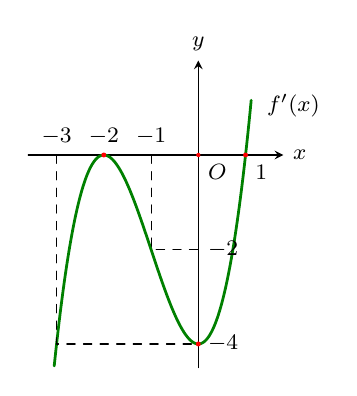
\begin{tikzpicture}[scale=0.6,line join=round,line cap=round,>=stealth,font=\footnotesize]
			% Axes
			\draw[->] (-3.6,0)--(1.8,0) node[right] {$x$};
			\draw[->] (0,-4.5)--(0,2) node[above] {$y$};
			
			% Graph y=(x+2)^2(x-1)
			\draw[green!50!black,line width=1pt,smooth,samples=200,domain=-3.05:1.12]
			plot (\x,{(\x+2)^2*(\x-1)});
			
			% Dashed guides
			\draw[dashed] (-3,0)--(-3,-4)--(0,-4);
			\draw[dashed] (-1,0)--(-1,-2)--(0,-2);
			
			% Points
			\fill[red] (-2,0) circle (1.5pt);
			\fill[red] (1,0) circle (1.5pt);
			\fill[red] (0,-4) circle (1.5pt);
			\fill[red] (0,0) circle (1.3pt);
			
			% Labels
			\node[above] at (-3,0) {$-3$};
			\node[above] at (-2,0) {$-2$};
			\node[above] at (-1,0) {$-1$};
			\node[below right] at (0,0) {$O$};
			\node[below right] at (1,0) {$1$};
			\node[right] at (0,-2) {$-2$};
			\node[right] at (0,-4) {$-4$};
			\node[right] at (1.25,1.05) {$f'(x)$};
		\end{tikzpicture}
	}
	\loigiai{
		\begin{itemchoice}
			\itemch Dựa vào đồ thị, ta có
			\begin{center}
				
\begin{tikzpicture}[scale=1,font=\footnotesize,line join=round
					,line cap=round,>=stealth]
					\tkzTabInit[nocadre=false,lgt=1.2,espcl=3, deltacl=0.5]
					{$x$/0.6,$f'(x)$/0.6}
					{$-\infty$,$-2$,$1$,$+\infty$}
					\tkzTabLine{,-,0,-,0,+,}
				\end{tikzpicture}
			\end{center}
			Vậy hàm số $f(x)$ chỉ có một điểm cực trị.
			\itemch
			\immini{Điều kiện xác định của hàm số
				$g(x)=\dfrac{\sqrt{x}}{f'(x)+2}$
				là $x\ge 0$ và $f'(x)+2\ne 0$.\\
				Từ đồ thị, phương trình $f'(x)=-2$
				chỉ có một nghiệm dương, gọi là $x_0$.\\
				Ta có $\lim\limits_{x\to x_0}\left(f'(x)+2\right)=0$ và
				$\lim\limits_{x\to x_0}\sqrt{x}=\sqrt{x_0}>0$.\\
				Do đó $\lim\limits_{x\to x_0^-}\dfrac{\sqrt{x}}{f'(x)+2}=-\infty$; $\lim\limits_{x\to x_0^+}\dfrac{\sqrt{x}}{f'(x)+2}=+\infty$.\\
				Vậy đồ thị hàm số $g(x)$ chỉ có đúng một tiệm cận đứng.
			}{
				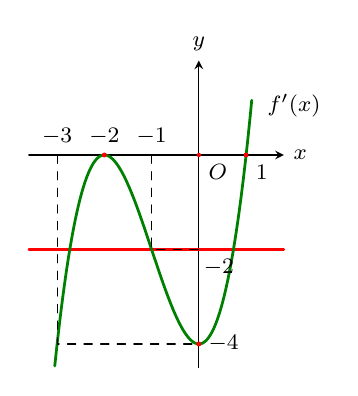
\begin{tikzpicture}[scale=0.6,line join=round,line cap=round,>=stealth,font=\footnotesize]
					\draw[->] (-3.6,0)--(1.8,0) node[right] {$x$};
					\draw[->] (0,-4.5)--(0,2) node[above] {$y$};
					\draw[red,thick] (-3.6,-2)--(1.8,-2);
					\draw[green!50!black,line width=1pt,smooth,samples=200,domain=-3.05:1.12]
					plot (\x,{(\x+2)^2*(\x-1)});
					\draw[dashed] (-3,0)--(-3,-4)--(0,-4);
					\draw[dashed] (-1,0)--(-1,-2)--(0,-2);
					\fill[red] (-2,0) circle (1.5pt);
					\fill[red] (1,0) circle (1.5pt);
					\fill[red] (0,-4) circle (1.5pt);
					\fill[red] (0,0) circle (1.3pt);
					\node[above] at (-3,0) {$-3$};
					\node[above] at (-2,0) {$-2$};
					\node[above] at (-1,0) {$-1$};
					\node[below right] at (0,0) {$O$};
					\node[below right] at (1,0) {$1$};
					\node[below right] at (-0.1,-2) {$-2$};
					\node[right] at (0,-4) {$-4$};
					\node[right] at (1.25,1.05) {$f'(x)$};
				\end{tikzpicture}
			}
			\itemch Dựa vào đồ thị ta thấy $f'(x)>0$, $\forall x\in(1;+\infty)$ suy ra $f'(x)>0$, $\forall x\in(2;+\infty)$ .\\
			Vậy hàm số $f(x)$ đồng biến trên khoảng $(2;+\infty)$.
			\itemch Từ đồ thị ta thấy $f'(x)=0$ tại $x=-2$ và $x=1$.\\
			Do đồ thị tiếp xúc trục hoành tại $x=-2$ nên $-2$ là nghiệm kép của $f'(x)$.\\
			Suy ra $f'(x)=a(x+2)^2(x-1)$.\\
			Mặt khác, từ đồ thị có $f'(0)=-4$, nên $-4a=-4\Rightarrow a=1$.\\
			Do đó $f'(x)=(x+2)^2(x-1)=x^3+3x^2-4$.\\
			Vậy $f'(2)=(2+2)^2(2-1)=16$.
		\end{itemchoice}
	}
\end{ex}
\Closesolutionfile{ans}

\caukq
\Opensolutionfile{ans}[ans/ans-19-26-2-DaNang-LienTruong-L1-KQ]
%%%=============EX_17=============%%%
\begin{ex}%[1D7C2-8]%[TEX ĐỀ THI THỬ THPT 2026]%[NGUYỄN VĂN HIỆP]
	\immini[thm]{Một cái bể nước hình nón để ngược như hình vẽ, có chiều cao $51$ cm, bán kính đáy bằng $50$ cm. Một vòi nước chảy vào bể sao cho sau mỗi giây chiều cao mực nước tăng đều lên $2$ cm cho đến khi đầy bể. Hãy tính tốc độ tăng thể tích (m$^3$/s) của nước trong khoảng thời gian một giây ngay trước khi bể đầy. ({\it Kết quả làm tròn đến hàng phần trăm}).
	}{
		\begin{tikzpicture}[scale=1,>=stealth, font=\footnotesize, line join=round, line cap=round]
			\def\h{-3}
			\def\a{2}
			\def\b{.5}
			\begin{scope}%thiết diện vuông góc với trục
				\path
				(0,-4) coordinate (O)
				%($(O)+(\a,0)$) coordinate (B)
				($(O)+(0,\h)$) coordinate (S)
				($(O)!0.4!(S)$) coordinate (O')
				($(O)+(0:\a cm and \b cm)$) coordinate (A)
				($(S)+(0:\a cm and \b cm)$) coordinate (B)
				($(O)+(-10:\a cm and \b cm)$) coordinate (M)
				($(O)+(190:\a cm and \b cm)$) coordinate (N)
				($(O')+(10:0.6*\a cm and 0.6*\b cm)$) coordinate (M')
				($(O')+(170:0.6*\a cm and 0.6*\b cm)$) coordinate (N')
				;
				\fill[cyan!50] (S)--(M')--(N')--cycle;
				\fill[cyan!30] (M') arc (10:170:0.6*\a cm and 0.6*\b cm)--(M') arc (10:-190:0.6*\a cm and 0.6*\b cm);
				\draw (O) ellipse (\a cm and \b cm );
				\draw [dashed] (M') arc (10:170:0.6*\a cm and 0.6*\b cm);
				\draw (M') arc (10:-190:0.6*\a cm and 0.6*\b cm);
				\draw (N)--(S)--(M);
				\draw [dashed] (S)--(O);
				\draw[<->] (O)--(A) node[pos=0.5,above]{$50$ cm}; 
				\draw[<->] (A)--(B) node[pos=0.5,right]{$51$ cm}; 
			\end{scope}
		\end{tikzpicture}
	}
	%\par\shortans[0]{0,02}
	\loigiai{
		Gọi $H=51$ (cm) là chiều cao của bể hình nón và $R=50$ (cm) là bán kính đáy của bể. \\
		Gọi $h$ (cm) là chiều cao mực nước và $r$ (cm) là bán kính mặt nước tại chiều cao $h$. \\
		Ta có $\dfrac{r}{h}=\dfrac{R}{H}\Rightarrow r=\dfrac{R}{H}h=\dfrac{50}{51}h$. \\
		Thể tích nước trong bể khi mực nước có chiều cao $h$ là $V=\dfrac{1}{3}\pi r^2h=\dfrac{1}{3}\pi\left(\dfrac{50}{51}h\right)^2h=\dfrac{2\,500\pi}{7\,803}h^3$. \\
		Vì mỗi giây mực nước tăng đều $2$ cm, nên chiều cao mực nước thời gian một giây ngay trước khi bể đầy là
		\[h_0 = 51 - 2 = 49 \;\text{(cm)}.\]
		Tốc độ tăng thể tích trong khoảng thời gian $1$ giây này chính là lượng thể tích nước tăng thêm từ lúc $h_0=49$ (cm) đến khi $h=51$ (cm).\\
		Vậy lượng thể tích tăng của nước trong khoảng thời gian một giây ngay trước khi bể đầy là
		\[\Delta V=V(51)-V(49)= \dfrac{2\,500\pi}{7\,803}(51^3-49^3)= \dfrac{2\,500\pi \cdot 15\,002}{7\,803} \, \left(\text{cm}^3\right).\]
		Ta có $\dfrac{2\,500\pi\cdot 15\,002}{7\,803}$ cm$^3$ $=\dfrac{2\,500\pi\cdot 15\,002}{7\,803\cdot 10^6}\approx 0{,}02$ m$^3$.\\
		Vậy tốc độ tăng thể tích của nước trong khoảng thời gian một giây ngay trước khi bể đầy khoảng $0{,}02$ (m$^3$/s).
	}
\end{ex}
%%%=============================%%%

%%%=============EX_18=============%%%
\begin{ex}%[2H2V2-2]%[TEX ĐỀ THI THỬ THPT 2026]%[NGUYỄN VĂN HIỆP]
	Trong không gian với hệ trục tọa độ $Oxyz$ cho hình thang $ABCD$ vuông tại $A$ và $B$. Biết $A(1;2;1)$, $B(2;0;3)$, $C(6;1;2)$ và hình thang có diện tích bằng $12\sqrt{2}$. Giả sử đỉnh $D(a;b;c)$, tìm $a+b+c$ ? ({\it Làm tròn kết quả đến chữ số hàng phần chục}).
	%\par\shortans[0]{10,7}
	\loigiai{
		\immini{
			Ta có\\
			$\overrightarrow{AB}=(1;-2; 2)\Rightarrow AB=\sqrt{1^2+(-2)^2+2^2}=3$. \\
			$\overrightarrow{BC}=(4; 1;-1)\Rightarrow BC=\sqrt{4^2+1^2+(-1)^2}=3\sqrt{2}$. \\
			Đặt $AD=x$ ($x>0$). Khi đó\\
			Hình thang $ABCD$ vuông tại $A$ và $B$ có diện tích là
			\[S=\dfrac{(AD+BC)\cdot AB}{2}=\dfrac{\left(x+3\sqrt{2}\right)\cdot3}{2}.\]
		}{
			\begin{tikzpicture}[scale=1,>=stealth, font=\footnotesize, line join=round, line cap=round]
				\def\a{3} \def\b{4.5} \def\h{2.5}
				\path 
				(0,0) coordinate (A)++(0:\b) coordinate (D)
				(A)++(90:\h) coordinate (B)++(0:\a) coordinate (C)
				;
				\draw (A)--(B)--(C)--(D)--cycle;
				\draw pic[draw,angle radius=2mm]{right angle=D--A--B};
				\foreach \x/\g in {A/-150,B/150,C/30,D/-30}
				\fill[black] (\x) circle (1pt)
				($(\g:3mm)+(\x)$) node {$\x$};
			\end{tikzpicture}
		}
		\noindent
		Theo đề bài ta có $S=12\sqrt{2}\Rightarrow\dfrac{\left(x+3\sqrt{2}\right)\cdot3}{2}=12\sqrt{2}\Leftrightarrow x=5\sqrt{2}$.\\
		Vì $\overrightarrow{AD}$ cùng hướng với $\overrightarrow{BC}$, nên $\overrightarrow{AD}=k\overrightarrow{BC}$ với $k>0$.\\
		Suy ra $AD=k\cdot BC\Rightarrow 5\sqrt{2}=k\cdot 3\sqrt{2}\Rightarrow k=\dfrac{5}{3}$.\\
		$\Rightarrow\overrightarrow{AD}=\dfrac{5}{3}\overrightarrow{BC}
		\Leftrightarrow
		\heva{
			&a-1=\dfrac{5}{3}\cdot 4\\
			&b-2=\dfrac{5}{3}\cdot1\\
			&c-1=\dfrac{5}{3}\cdot(-1)}
		\Leftrightarrow
		\heva{
			&a=\dfrac{23}{3}\\&b=\dfrac{11}{3}\\&c=-\dfrac{2}{3}}
		\Rightarrow
		a+b+c=\dfrac{23}{3}+\dfrac{11}{3}-\dfrac{2}{3}\approx10{,}7$.
	}
\end{ex}
%%%=============================%%%

%%%=============EX_19=============%%%
\begin{ex}%[2H2H2-6]%[TEX ĐỀ THI THỬ THPT 2026]%[NGUYỄN VĂN HIỆP]
	\immini[thm]{Trong không gian với một hệ trục tọa độ $Oxyz$ cho trước (mặt phẳng $(Oxy)$ trùng với mặt đất, trục $Oz$ hướng thẳng đứng lên trời, đơn vị đo trên mỗi trục lấy theo kilomét), một chiếc máy bay đang di chuyển với hướng bay không đổi từ điểm $M(-50;30;10)$ đến vị trí hạ cánh là $N(2;3;0)$. Đường bay của máy bay hợp với phương thẳng đứng một góc $a^\circ$. Tìm $a$? ({\it Làm tròn kết quả đến hàng đơn vị}).
	}{
%		\begin{tikzpicture}[scale=1,>=stealth, font=\footnotesize, line join=round, line cap=round]
%			\path (0,0) coordinate (O)
%			(-2,2) coordinate (A)
%			;
%			\tikzset{maybay/.pic={
%					\begin{scope}[line width=1pt,opacity=0.95,scale=.4,rotate=-12]
%						\fill[ball color =cyan!40!gray,,rounded corners=2mm](-5.6,3)--++(60:0.8)--++(2:0.55)--++(-90:2)--cycle;
%						%%Hai cánh
%						\fill[ball color =cyan!90!gray!40!white](-0.4,1.5)..controls++(75:2)and++(-68:0.75)..(-0.15,4)--++(-5:0.35)..controls++(-50:0.95)and++(106:2)..(1.25,1.5)--cycle;
%						%Thân
%						\fill[ball color =cyan!30!gray](-4.85,1)..controls++(-90:0.6) and++(180:0.2)..(-4,0.5)--++(-12:3.3)--++(0:4)..controls++(0:2) and++(-172:1)..(6,0)..controls++(8:1)and++(-90:0.1)..(6.85,0.3)..controls++(90:0.2) and++(-30:1)..(5,1.3)..controls++(90:0.25) and++(0:8)..(-4,1.5)--cycle;
%						\draw[cyan!40!black](6.85,0.3)..controls++(-90:0.5) and++(0:6)..(-2,0.2);
%						% Cánh phải
%						\fill[ball color =cyan!90!gray!40!white,rounded corners=2mm](-1.8,0)--++(-5:0.35)--++(-147:4.85)--++(-50:0.7)--++(25.5:6.5)..controls++(-155.5:0.5) and++(-170:0.15)..(1.5,-0.25)..controls++(120:0.5) and++(2:1)..(-1.8,0);
%						\fill[ball color =cyan!90!gray!40!white,rounded corners=2mm](-6.1,-2.3)--++(-54:0.7)--++(-28:0.7)--++(25.5:.35)--++(-180:.2)--++(135:1.2)--cycle;
%						%%Thân đuôi
%						\fill[ball color =cyan!90!gray!40!white,rounded corners=2mm](-6.9,3.6)--++(2:1)..controls++(-35:2) and++(178:2.3)..(-2,1.5)..controls++(-90:0.2) and++(20:1)..(-3.5,1)--++(180:1.2)--cycle;
%						%%Đuôi
%						\fill[ball color =cyan!90!gray!40!white,rounded corners=2mm](-6,2.5)--++(0:1.35)--++(-156:2.5)--++(170:0.75)--cycle;
%						\fill[ball color =cyan!70!gray!40!white,rounded corners=2mm](-1.9,-0.17)--++(90:0.72)--++(181:2.45)--++(-90:0.6)--cycle;
%						\fill[ball color =cyan!90!gray!10!black,line width=2pt,draw=cyan!30!black,rounded corners=0.5mm](-1.9,-0.18)arc(-90:270:0.2 and 0.38);
%						\fill[cyan](5.05,1.3)--++(-25:0.8)..controls++(-140:0.55)and++(10:0.5)..(4.2,0.6)..controls++(180:0.15) and++(182:0.45)..(4.3,1.1)..controls++(2:0.5) and++(-135:0.2)..(5.1,1.3);
%						\draw[draw=teal,double,distance=0.3mm](5.05,1.3)++(-26:0.8)..controls++(-140:0.55)and++(10:0.5)..(4.2,0.6)foreach \i in{1,2,...,4}{coordinate[pos=\i/4](B\i)}..controls++(180:0.15) and++(182:0.45)..(4.3,1.1)..controls++(2:0.5) and++(-135:0.2)..(5.1,1.3)foreach \i in{1,2,...,10}{coordinate[pos=\i/10](A\i)}(A2)--(B2)(A6)--(B1);
%						\foreach \i in {0,1,...,6}
%						\fill[ball color=cyan](-0.8+0.5*\i,0.4)arc(-90:270:0.1 and 0.2);
%						\fill[draw=cyan!10!teal,ball color=cyan!80!gray,rounded corners=1.5mm](3.2,-0.2)--++(95:0.9)--++(0:0.5)--++(-85:0.9)--cycle;
%						\begin{scope}[opacity=1]
%							\fill[ball color=orange](2.5,-0.15)arc(-90:270:0.2 and 0.1);
%							\fill[ball color=orange!50!red!50!white,rotate around={10:(6,0.25)}](6,0.25)arc(-90:270:0.2 and 0.1);
%						\end{scope}
%						\begin{scope}[opacity=0.4]
%							\fill[ball color=orange](2.5,-0.15)arc(-90:270:0.2 and 0.1);
%							\fill[ball color=orange!50!red!50!white,rotate around={10:(6,0.25)}](6,0.25)arc(-90:270:0.2 and 0.1);
%						\end{scope}
%					\end{scope}
%				}
%			}
%			\draw[->] (O)--++(-130:2) node[left]{$x$};
%			\draw[->] (O)--++(0:4) node[below]{$y$};
%			\draw[->] (O)--++(90:3) node[left]{$z$};
%			\fill[black] (O) circle (1pt) node[left]{$O$};
%			\draw[->,line width=2pt] (A)--++(-30:2);
%			\pic[scale=.4,rotate around={-20:(A)}] at (A) {maybay};
%		\end{tikzpicture}
	}
	%\par\shortans[0]{80}
	\loigiai{
		Vectơ chỉ phương của đường bay của máy bay là $\overrightarrow{u}=\overrightarrow{MN}=(52;-27;-10)$. \\
		Vectơ chỉ phương của phương thẳng đứng (trục $Oz$) là $\overrightarrow{k}=(0; 0; 1)$. \\
		Gọi $\alpha$ là góc giữa đường bay của máy bay và phương thẳng đứng.\\
		Ta có
		$\cos\alpha=\dfrac{\left|\overrightarrow{u}\cdot\overrightarrow{k}\right|}{\left|\overrightarrow{u}\right|\cdot\left|\overrightarrow{k}\right|}=\dfrac{\left|52\cdot0+(-27)\cdot0+(-10)\cdot1\right|}{\sqrt{52^2+(-27)^2+(-10)^2}\cdot\sqrt{0^2+0^2+1^2}}=\dfrac{10}{\sqrt{3\,533}}$. \\
		Suy ra $\alpha\approx 80^\circ$
	}
\end{ex}
%%%=============================%%%

%%%=============EX_20=============%%%
\begin{ex}%[1H8V5-3]%[TEX ĐỀ THI THỬ THPT 2026]%[NGUYỄN VĂN HIỆP]
	Cho hình chóp $S.ABCD$ có đáy $ABCD$ là hình thoi tâm $O$, cạnh $a$, $\widehat{ABC}=60^\circ$. Biết rằng $SO\perp(ABCD)$, $SO=\dfrac{3a}{2}$. Khoảng cách từ $A$ đến mặt phẳng $(SCD)$ bằng $\dfrac{ma\sqrt{13}}{n}$ với $\dfrac{m}{n}$ là phân số tối giản, $m>0$, $n>0$. Giá trị $m+n$ bằng bao nhiêu?
	%\par\shortans[0]{16}
	\loigiai{
		\immini{
			Ta có $ABCD$ là hình thoi tâm $O$ cạnh $a$, $\widehat{ABC}=60^\circ$.\\
			Suy ra $\triangle ACD$ đều cạnh $a$.\\
			Gọi $I$ là trung điểm $CD$, $M$ là trung điểm $IC$.\\
			Khi đó $AI=\dfrac{a\sqrt{3}}{2}$, $OM=\dfrac{AI}{2}=\dfrac{a\sqrt{3}}{4}$.\\
			Do $\triangle ADC$ đều nên $AI\perp CD\Rightarrow OM\perp CD$.\\
			Ta có $\heva{& CD\perp SO\\& CD\perp OM}\Rightarrow CD\perp(SOM)$\\
			Suy ra $ CD\perp OH\subset(SOM)$.
		}{
			\begin{tikzpicture}[scale=1,>=stealth, font=\footnotesize, line join=round, line cap=round]
				\def\a{3.5}
				\def\h{3.5}
				\path (0:0) coordinate (A)
				++(0:\a) coordinate (D)
				++(-135:\a/2) coordinate (C)
				($(A)+(C)-(D)$) coordinate (B)
				(intersection of A--C and B--D) coordinate (O)
				($(O)+(90:\h)$) coordinate (S)
				($(C)!.5!(D)$) coordinate (I)
				($(C)!.5!(I)$) coordinate (M)
				($(S)!.65!(M)$) coordinate (H)
				;
				\draw[dashed] (B)--(A)--(D)(A)--(S) (A)--(I) (O)--(M) (O)--(H)
				(A)--(C)(B)--(D)(S)--(O);
				\draw(B)--(C)--(D) (B)--(S)(C)--(S) (D)--(S) --(M);
				\foreach \x/\g in {A/135,B/-135,C/-45,D/45,S/90,O/-90,M/-30,I/0,H/30}
				\fill[black] (\x) circle (1pt)
				($(\g:2.5mm)+(\x)$) node {$\x$};
				\draw pic[draw,angle radius=2mm]{right angle=O--M--C};
				\draw pic[draw,angle radius=2mm]{right angle=A--I--C};
			\end{tikzpicture}
		}
		\noindent
		Ta có $\heva{&OH\perp SM\subset(SCD)\\& OH\perp CD}\Rightarrow OH\perp(SCD)\Rightarrow\mathrm{d}\big(O,(SCD)\big)=OH$.\\
		Tam giác $SOM$ vuông tại $O$, $OH\perp SM$ tại $H$.\\
		Suy ra $\dfrac{1}{OH^2}=\dfrac{1}{OM^2}+\dfrac{1}{SO^2}=\dfrac{16}{3a^2}+\dfrac{4}{9a^2}=\dfrac{52}{9a^2}\Rightarrow OH=\dfrac{3a\sqrt{13}}{26}$.\\
		Ta có $AO\cap(SCD)=C$ và $AC=2OC$.\\
		Suy ra
		$\mathrm{d}\big(A,(SCD)\big)=2\mathrm{d}\big(O,(SCD)\big)=2OH=2\cdot\dfrac{3a\sqrt{13}}{26}=\dfrac{3a\sqrt{13}}{13}=\dfrac{ma\sqrt{13}}{n}$.\\
		Do đó $m=3$, $n=13$. Suy ra $m+n=3+13=16$.
	}
\end{ex}
%%%=============================%%%

%%%=============EX_21=============%%%
\begin{ex}%[1D2V3-8]%[TEX ĐỀ THI THỬ THPT 2026]%[NGUYỄN VĂN HIỆP]
	Để chuẩn bị cho hành trình học đại học sau khi tốt nghiệp phổ thông, ngay từ đầu năm lớp $10$, được sự đồng ý của cha mẹ, bạn Hùng vừa đi học vừa đi làm thêm để có thể giảm gánh nặng kinh tế cho gia đình. Tháng đầu tiên đi làm, bạn Hùng được ông chủ trả $3$ triệu đồng, nhờ siêng năng làm việc nên cứ mỗi tháng ông chủ lại tăng $7\%$ lương so với tiền lương tháng liền trước. Mỗi khi lĩnh lương, bạn Hùng đều cất đi phần lương tăng so với tháng trước. Hỏi sau $3$ năm kể từ khi bắt đầu đi làm thêm thì bạn Hùng tiết kiệm được bao nhiêu triệu đồng? ({\it Làm tròn kết quả đến chữ số hàng đơn vị}).
	%\par\shortans[0]{29}
	\loigiai{
		\begin{itemize}
			\item Gọi $L_n$ là số tiền lương bạn Hùng nhận được trong tháng thứ $n$ (đơn vị triệu đồng). \\
			Theo đề bài, tháng đầu tiên bạn Hùng nhận được $3$ triệu đồng, nên $L_1=3$. \\
			Mỗi tháng, lương tăng $7\%$ so với tháng liền trước, nên ta có $L_n=L_{n-1}\cdot(1+0{,}07)=L_{n-1}\cdot 1{,}07$. \\
			Từ đó, công thức tổng quát cho lương tháng thứ $n$ là $L_n=L_1\cdot(1{,}07)^{n-1}=3\cdot(1{,}07)^{n-1}$.
			\item Gọi $S_n$ là số tiền tiết kiệm được trong tháng thứ $n$. \\
			Tháng đầu tiên ($n=1$), số tiền tăng so với tháng trước là $0$. \\
			Tháng thứ $n$ ($n\ge 2$), số tiền tăng so với tháng trước là
			\[S_n=L_n - L_{n-1}=L_1 \cdot (1{,}07)^{n-1} - L_1 \cdot (1{,}07)^{n-2}= L_1 \cdot (1{,}07)^{n-2}\cdot 0{,}07=0{,}21\cdot (1{,}07)^{n-2}.\]
			\item
			Thời gian bạn Hùng đi làm là $3$ năm, tương ứng với $3\cdot 12=36$ tháng. \\
			Tổng số tiền bạn Hùng tiết kiệm được sau $36$ tháng là tổng của các khoản tiết kiệm từ tháng thứ $2$ đến tháng thứ $36$.
			\allowdisplaybreaks
			\begin{eqnarray*}
				S&=&S_2+ S_3 + \cdots + S_{36}\\
				&=& 0{,}21\cdot 1 + 0{,}21\cdot (1{,}07)+ 0{,}21\cdot (1{,}07)^2+\cdots + 0{,}21\cdot (1{,}07)^{34}\\
				&=& 0{,}21\cdot\left[1+(1{,}07) + (1{,}07)^2+ \cdots + (1{,}07)^{34}\right]\\
				&=& 0{,}21\cdot \dfrac{1-(1{,}07)^{35}}{1-1{,}07}\\
				&\approx& 29.
			\end{eqnarray*}
		\end{itemize}
		Vậy, sau $3$ năm bạn Hùng tiết kiệm được khoảng $29$ triệu đồng.
		
	}
\end{ex}
%%%=============================%%%

%%%=============EX_22=============%%%
\begin{ex}%[2D1V5-6]%[TEX ĐỀ THI THỬ THPT 2026]%[NGUYỄN VĂN HIỆP]
	\immini[thm]{Có một hòn đảo nằm trong một vịnh biển, giả sử rằng đường bao sát biển của hòn đảo được mô hình hóa vào hệ trục tọa độ $Oxy$ là một phần bên phải trục tung của đồ thị hàm số bậc ba $y=f(x)=-x^3+3x^2+2$ và giả sử một con đường trong đất liền chạy trên một đường thẳng có phương trình là $y=-9x+60$ như hình vẽ, với đơn vị trên mỗi trục tọa độ là $100$ m. Tập đoàn đầu tư du lịch ST muốn làm một cây cầu vuợt biển có dạng một đoạn thẳng nối từ con đường trong đất liền ra hòn đảo để khai thác du lịch sinh thái. Tính độ dài ngắn nhất (đơn vị mét) của cây cầu cần làm? ({\it Làm tròn kết quả đến chữ số hàng đơn vị}).
	}{
		\begin{tikzpicture}[xscale=.5,yscale=.6,>=stealth, font=\footnotesize, line join=round, line cap=round]
			\def\a{-1} \def\b{3} \def\c{0} \def\d{2} % Hệ số
			\def\xmin{-1} \def\xmax{7.5}
			\def\ymin{-1} \def\ymax{7} 
			%\draw[color=gray!50,dashed] (\xmin,\ymin) grid (\xmax,\ymax); 
			\draw[->] (\xmin,0)--(\xmax,0) node [below]{$x$};
			\draw[->] (0,\ymin)--(0,\ymax) node [left]{$y$};
			\node at (0,0) [below left]{$O$};
			\clip (\xmin+0.1,\ymin+0.1) rectangle (\xmax-0.5,\ymax-0.1);
			\draw[smooth,samples=300,thick] plot[domain=0:4](\x,{\a*(\x)^3+\b*(\x)^2+\c*(\x)+\d});
			\draw[smooth,samples=300,domain=4.5:6.5,thick]plot(\x,{-9*(\x)+50});
			\node at (1.5,2){Hòn đảo};
			\node [] at (6,6){Đường đất};
			\node [rotate=-80] at (5.5,4){$y=-9x+60$};
			\node at (2,6.5){$y=f(x)$};
		\end{tikzpicture}
	}
	%\par\shortans[0]{342}
	\loigiai{
		\immini{
			Gọi $M(x_0;y_0)$ với ($x_0>0$) là điểm thuộc đồ thị hàm số $y=f(x)$. \\
			Cây cầu vuợt biển là một đoạn thẳng nối từ con đường trong đất liền ra hòn đảo tại điểm $M$ ngắn nhất khi tiếp tuyến của đồ thị hàm số $y=f(x)$ tại điểm $M$ song song với đường thẳng $d\colon y=-9x+60$. Khi đó
			\allowdisplaybreaks
			\begin{eqnarray*}
				f'(x_0)=-9&\Leftrightarrow& -3x_0^2+6x_0=-9 \\
				&\Leftrightarrow& -3x_0^2+6x_0+9=0\\
				&\Leftrightarrow&\hoac{&x_0=-1~\text{(loại)}\\&x_0=3~\text{(nhận)}.}
			\end{eqnarray*}
		}{
			\begin{tikzpicture}[xscale=.8,yscale=.6,>=stealth, font=\footnotesize, line join=round, line cap=round]
				\def\a{-1} \def\b{3} \def\c{0} \def\d{2} % Hệ số
				\def\xmin{-1} \def\xmax{7.5}
				\def\ymin{-1} \def\ymax{7} 
				%\draw[color=gray!50,dashed] (\xmin,\ymin) grid (\xmax,\ymax); 
				\draw[->] (\xmin,0)--(\xmax,0) node [below]{$x$};
				\draw[->] (0,\ymin)--(0,\ymax) node [left]{$y$};
				\node at (0,0) [below left]{$O$};
				\clip (\xmin+0.1,\ymin+0.1) rectangle (\xmax-0.5,\ymax-0.1);
				\draw[smooth,samples=300,thick] plot[domain=0:4](\x,{\a*(\x)^3+\b*(\x)^2+\c*(\x)+\d});
				\draw[smooth,samples=300,domain=4.5:6.5,thick]plot(\x,{-9*(\x)+50});
				\draw[smooth,samples=300,domain=2:3.5,thick,dashed]plot(\x,{-9*(\x)+29});
				\node at (1.5,2){Hòn đảo};
				\node [] at (6,6){Đường đất};
				\node [rotate=-80] at (5.5,4){$y=-9x+60$};
				\node at (1.5,6.5){$y=f(x)$};
				\draw[fill=black] (3,2) circle (1pt) node[above right]{$M$};
				\draw[thick] (3,2)--++(10:2.3)node[below,sloped,pos=.5]{Cầu};
			\end{tikzpicture}
		}
		
		\noindent
		Với $x_0=3\Rightarrow f(x_0)=-3^3+3\cdot3^2+2=2\Rightarrow M(3; 2)$.\\
		Ta có $d\colon y=-9x+60\Leftrightarrow 9x+y-60=0$ là đường đất.\\
		Khoảng cách từ điểm $M(3; 2)$ đến đường thẳng $d$ là
		$\mathrm{d}\big(M,d\big)=\dfrac{\left|9\cdot3+2-60\right|}{\sqrt{9^2+1^2}}=\dfrac{31}{\sqrt{82}}$.\\
		Vì đơn vị trên mỗi trục tọa độ là $100$ m nên độ dài ngắn nhất của cây cầu là
		$\dfrac{31}{\sqrt{82}}\cdot100\approx 342$ m.
	}
\end{ex}

\Closesolutionfile{ans}

%\indapan{6}{ans/ans-19-26-2-DaNang-LienTruong-L1-LC}
%\indapan{4}{ans/ans-19-26-2-DaNang-LienTruong-L1-DS}
%\indapan{6}{ans/ans-19-26-2-DaNang-LienTruong-L1-KQ}
